\chapter{Descripción del hardware}\label{chp-02}

\lettrine[lraise=-0.1, lines=2, loversize=0.2]{U}na vez conocidas las funciones
que debe desempeñar el sistema es importante definir el hardware a usar para que
sea capaz de cumplimentar los requerimientos establecidos. Los principales dispositivos
utilizados en el proyecto son los siguientes:

\section{Arduino Mega 2560}

Se trata de una placa de desarrollo que cuenta con el microcontrolador ATmega2560 y todo lo
necesario para prototipar un sistema. Cuenta con 54 pines de entrada y salida (GPIO), de los cuales
15 pueden utilizarse como salida PWM, 4 puertos UART, oscilador de 16 MHz, conexión USB tipo B,
pines ICSP de programación y botón de reinicio.

\begin{figure}[hbtp]
	\centering
	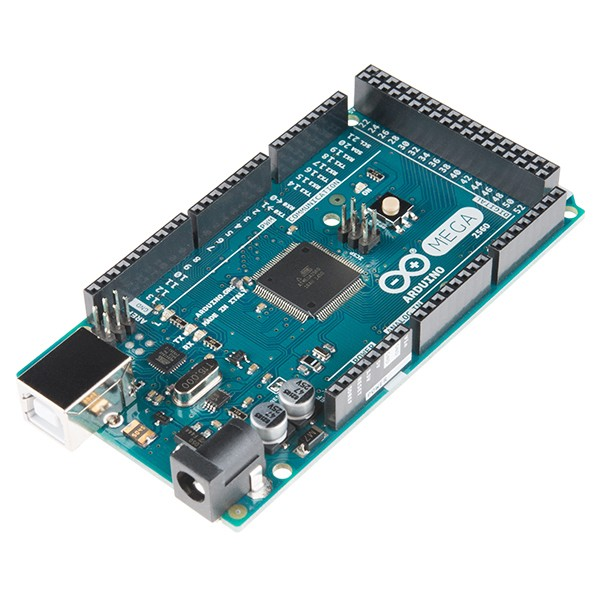
\includegraphics[scale=0.5]{02-hardware/01-arduino-mega-2560.jpg}
	\caption{Arduino Mega 2560}
	\label{fig:figura21}
	\end{figure}


\begin{table}[hbtp]
    \begin{center}
    \begin{tabular}{ | c | c |  }
    \hline
    Microcontrolador & ATmega2560 \\ \hline
    Tensión de funcionamiento & 5 V \\ \hline
    Voltaje de entrada recomendado & 7-12 V \\ \hline
    Voltaje de entrada límite & 6-20 V \\ \hline
    Pines de E/S digitales & 54 (de los cuales 15 con salida PWM) \\ \hline
    Pines de entrada analógica & 16 \\ \hline
    Corriente CC por pin & 20 mA \\ \hline
    Corriente CC para pin 3.3 V & 50 mA \\ \hline
    Memoria Flash & 256 kB, 8 kB utilizados por el gestor de arranque \\ \hline
    SRAM & 8 kB \\ \hline
    EEPROM & 4 kB \\ \hline
    Frecuencia de reloj & 16 MHz \\ \hline
    Longitud & 101.52 mm \\ \hline
    Anchura & 53.3 mm \\ \hline
    Peso & 37 g \\ \hline

    \end{tabular}
    \end{center}
    \caption{Características Arduino Mega 2560}
    \label{tab:tab1}
    \end{table}


\subsection{Alimentación}

El Arduino Mega 2560 puede ser alimentado mediante la conexión USB tipo B proporcionada por
un ordenador o por una fuente de alimentación externa. Además, puede ser alimentado por los pines
de alimentación de la placa, que se describen a continuación:

\begin{itemize}
    \item VIN. Entrada de tensión de la placa cuando hay alimentación externa.
    \item 5V. Pin que produce 5V regulados.
    \item 3V3. Pin que produce 3.3V regulados con un consumo máximo de 50 mA.
    \item GND. Pin de conexión a masa.
    \item IOREF. Referencia de tensión de trabajo del microcontrolador.
\end{itemize}

\subsection{Memoria}

El ATmega2560 cuenta con 256 kB de memoria flash de los cuales 8 kB se usan para el gestor de arranque,
8 kB de memoria SRAM y 4 kB de EEPROM.

\subsection{Entradas y Salidas}

El Arduino Mega cuenta con 54 pines que pueden ser utilizados como salida o entrada digital mediante
las funciones pinMode(), digitalWrite() y digitalRead(). Los niveles lógicos son de 5V. Cada pin soporta
una corriente de 20 mA y cuenta con una resistencia de pull-up de entre 20 y 50 k$\Omega$. Además, algunos pines
tienen funciones especiales:

\begin{itemize}
    \item Comunicación serie. Se usa para recibir y transmitir datos en serie TTL. Son las parejas 0 y 1,
    14 y 15, 16 y 17 y 18 y 19. Los pines 0 y 1 son los correspondientes a la comunicación con el conversor 
    USB-TTL integrado en la placa
    \item Interrupciones externas. Se utilizan para activar interrupciones en el software. Son los pines 2, 3, 18, 19, 20 y 21.
    \item Salida PWM. Proporcionan una salida modulada con 8 bits de precisión con la función analogWrite(). Son los pines del 
    2 al 13 y del 44 al 46.
    \item Comunicación SPI. Pines 50 (MISO), 51 (MOSI), 52 (SCK), 53 (SS). Permiten comunicación SPI con otros 
    dispositivos utilizando la biblioteca SPI.
    \item LED integrado. En el pin 13 hay un LED integrado que puede encenderse con un valor HIGH y apagarse con un valor LOW.
    \item Comunicación TWI. Pines 20 (SDA) y 21 (SCL). Permite comunicación I2C/TWI.
\end{itemize}

\subsection{Comunicación}

La placa Arduino Mega cuenta con diversas formas para comunicarse con un ordenador o con otros dispositivos. El ATmega2560
cuenta con cuatro UART de hardware para comunicación TTL a 5V, una conexión SPI y una conexión I2C. Mediante uno de los puertos
UART el ATmega2560 se comunica con un ATmega16U2 que canaliza la conexión mediante USB a un ordenador y permite la comunicación
entre ambos. Esto permite tanto programar la placa mediante el IDE de Arduino como recibir mediante monitor serie datos simples.

\section{Ethernet Shield de Arduino}

El Ethernet Shield de Arduino se trata de una placa que añade
la funcionalidad de conectar una placa de Arduino a una red 
mediante conexión Ethernet. Se trata de una placa basada en
el chip Wiznet W5100 que provee de una pila de red IP capaz de
soportar protocolos TCP y UDP. Usa la librería Ethernet para leer y 
escribir flujos de datos.

\begin{figure}[hbtp]
	\centering
	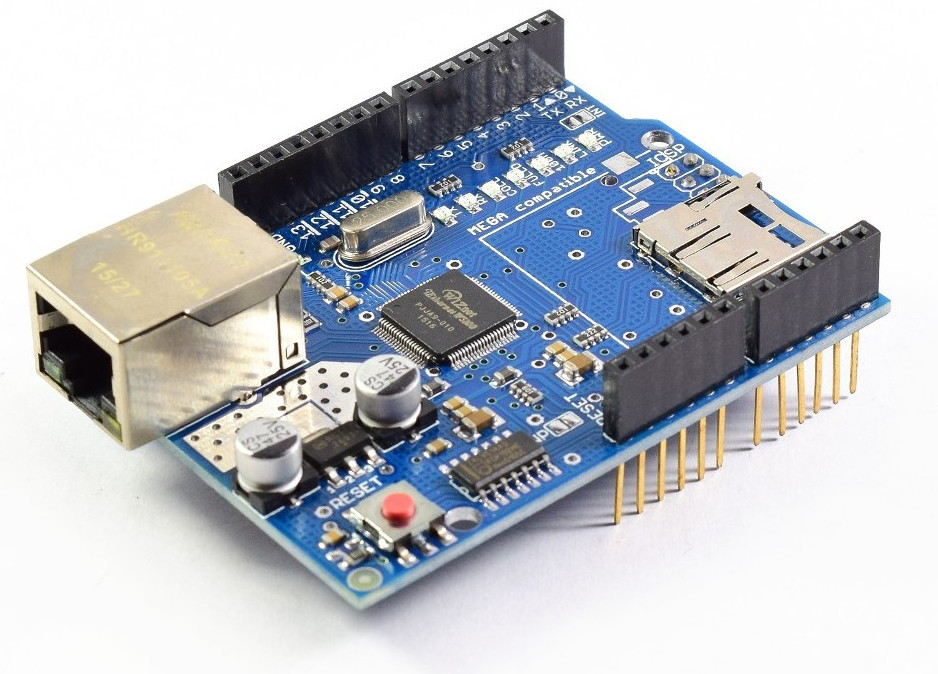
\includegraphics[scale=1]{02-hardware/02-shield-ethernet-w5100.jpg}
	\caption{Arduino Ethernet Shield}
	\label{fig:figura22}
	\end{figure}

La placa cuenta con varios LED que proporcionan información:
\begin{itemize}
    \item ON. Indica que la placa está alimentada.
    \item LINK. Indica presencia de enlace de red.
    \item 100M. Indica la existencia de conexión de red de 100 Mb/s.
    \item RX. Indica que se reciben datos cuando parpadea.
    \item TX. Indica que se transmiten datos cuando parpadea.
\end{itemize}

Unos puntos importantes del Ethernet Shield son:
\begin{itemize}
    \item Funciona a 5V.
    \item Tiene un microcontrolador W5100 con 16k de buffer y 
    es independiente de la memoria del ATmega2560.
    \item Se comunica con el ATmega2560 mediante SPI.
    \item Soporta 4 conexiones simultáneas.
    \item Utiliza la librería Ethernet.
    \item Dispone de lector de tarjetas microSD para guardar ficheros.
    \item Utiliza los pones 10, 11, 12 y 13 para comunicarse con el
    W5100 mediante SPI.
\end{itemize}

\section{Motor DC y Driver L298N}

El principal actuador de este proyecto es un motor de corriente
continua que es el que mueve la cinta transportadora, permitiéndola
avanzar, retroceder o pararse. Este motor funciona a 24V y tiene 
infinidad de uso, ya que son sencillos de operar y tienen un bajo coste.

Para controlar dicho motor se utiliza un Driver L298N, que está basada
en un puente H. Dicho módulo es capaz de controlar dos motores de 
corriente continua o un motor paso a paso bipolar de hasta 2A.

\begin{figure}[hbtp]
	\centering
	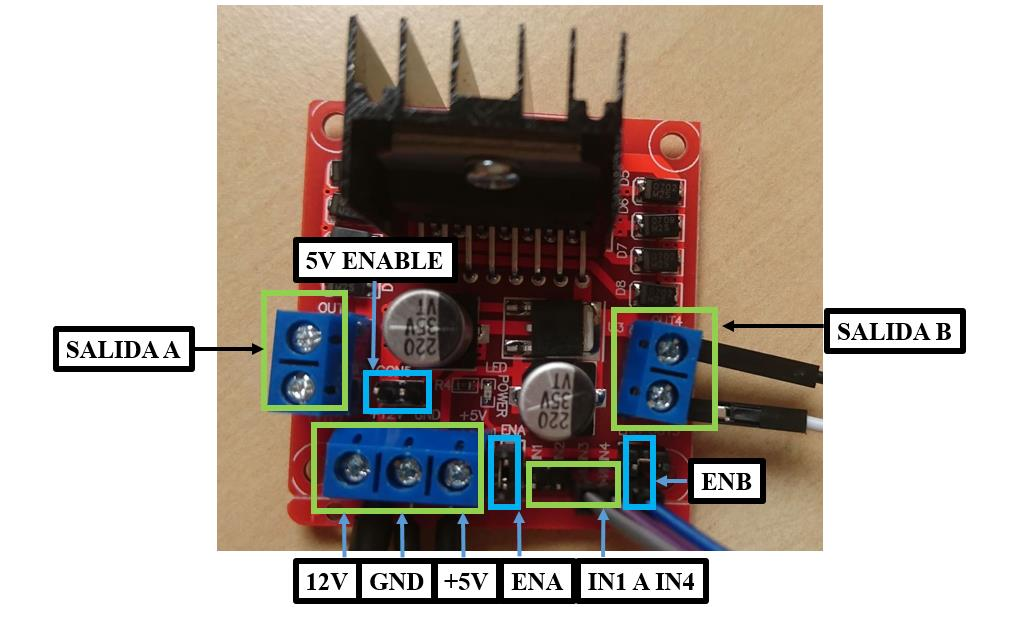
\includegraphics[scale=0.25]{02-hardware/03-l298n.png}
	\caption{Driver L298N}
	\label{fig:figura23}
	\end{figure}

La principal funcionalidad del módulo es separar la parte asociada
a la potencia (que funciona a 24V en este caso) de la parte asociada
al control (que funciona a 5V).

\subsection{Conexionado del módulo L298N}

El módulo cuenta con un circuito integrado LM7805 que proporciona 5V
que puede ser activado o desactivado mediante un jumper.

Mientras el jumper esté activo, la placa admite tensiones de 
alimentación de entre 6 y 12V. Así, la conexión de 5V será una salida.

Por otra parte, si el jumper está desactivado la placa admite tensiones
de alimentación de entre 12 y 35V. En este caso se deberá proporcionar
5V de referencia a la placa para el funcionamiento de la parte lógica.

\begin{figure}[hbtp]
	\centering
	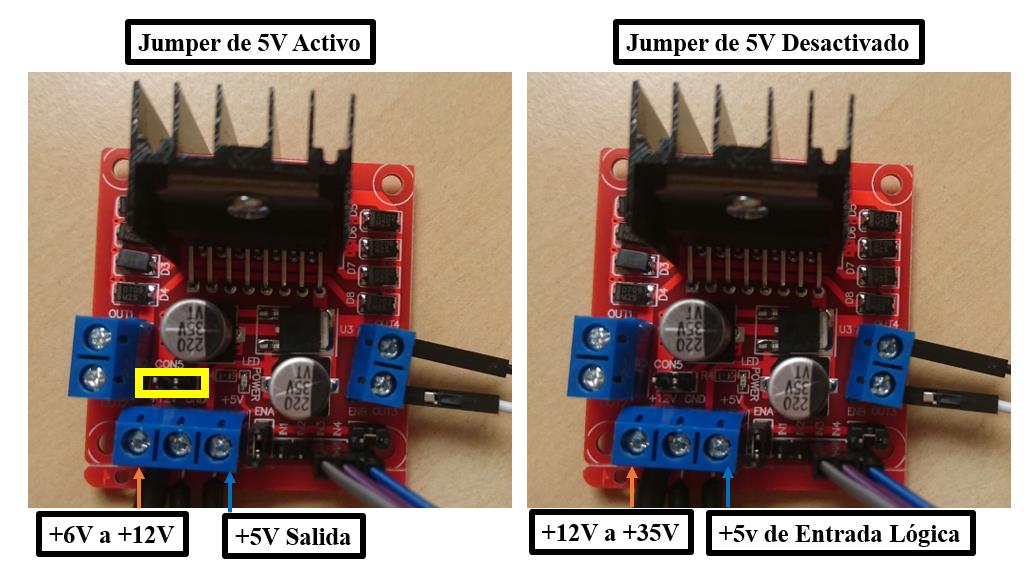
\includegraphics[scale=0.3]{02-hardware/04-l298n-alimentacion.png}
	\caption{Tipos de conexiones del Driver L298N}
	\label{fig:figura24}
	\end{figure}

\section{Encoder Rotativo Incremental}

Para posicionar correctamente las piezas a lo largo de la cinta es
necesario contabilizar el movimiento de la misma. Para ello, se cuenta
con un encoder rotativo incremental de serie LPD3806-600BM el cual
cuenta con una gran precisión.

Éste tiene dos salidas de onda cuadrada con un desfase de 90 grados
entre ellas. Siempre que se produzca un flanco en A, será leída la 
señal B. Si B se encuentra en HIGH, el encoder se encontrará girando
en sentido horario. Por el contrario, si B se encuentra en LOW, el 
encoder se encontrará girando en sentido antihorario. 

\begin{figure}[hbtp]
	\centering
	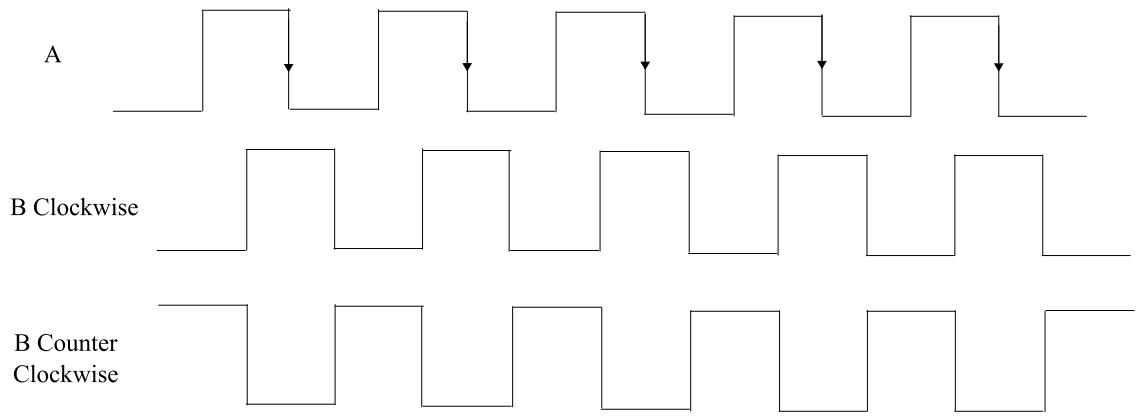
\includegraphics[width=\textwidth]{02-hardware/05-encoder.jpg}
	\caption{Señales encoder rotativo}
	\label{fig:figura25}
	\end{figure}

\subsection{Especificaciones técnicas}

El encoder rotativo de serie LPD3806-600BM cuenta con las
siguientes especificaciones:
\begin{itemize}
    \item 600 pulsos/revolución por cada fase. Por lo tanto, con las
    fases combinadas se cuenta con 2400 pulsos/revolución.
    \item Velocidad máxima: 5000 revoluciones/minuto.
    \item Respuesta de frecuencia: 0-30KHz
\end{itemize}

\subsection{Conexionado del Encoder}

El encoder cuenta con cuatro cuables de conexión:
\begin{itemize}
    \item Rojo. Alimentación 5-24V.
    \item Negro. GND.
    \item Verde. Fase A.
    \item Blanco. Fase B.
\end{itemize}

\section{Calibre digital}

Para tomar la medida de la posición a lo ancho de la cinta se utiliza
un calibre digital. Este instrumento se encuentra integrado en las
cintas transportadoras del laboratorio. Cuentan con un LCD en el que
se muestra la información de la medición y, además, cuenta con una tapa 
desmontable a la que se acceden cuatro pines que permiten comuncaciones
con el Arduino. Estos pines son: alimentación a 1.5V, GND, señal de 
reloj y señal de datos. Todas las señales utilizan un nivel lógico de 
tensión de 1.5V, por lo que deben ser amplificadas a 5V para que el 
Arduino pueda comprender dichas señales.

\begin{figure}[hbtp]
	\centering
	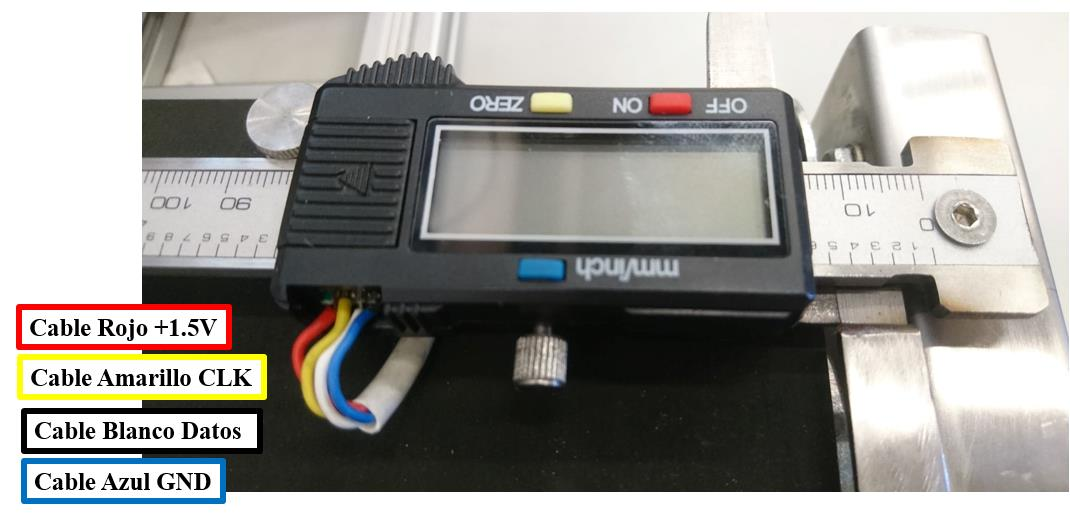
\includegraphics[width=\textwidth]{02-hardware/06-calibrador.png}
	\caption{Calibre digital y cables usados}
	\label{fig:figura26}
	\end{figure}


Mientras el calibre cuente con alimentación estará enviando tramas de
datos con la medida de cada momento, por lo que es recomendable no 
utilizar pilas ya que siempre está funcionando. Algunas características 
importantes son:

\begin{itemize}
    \item Cada trama cuenta con 24 bits, de los cuales 21 corresponden
    a la medición, uno para el signo, uno para la unidad (mm o in) y otro
    bit de acarreo.
    \item Los datos se transmiten por una señal de reloj (CLK) y una señal
    de datos (DATA).
    \item La línea de datos debe leerse en cada flanco de bajada de 
    la señal de reloj.
    \item Los bits de la trama se inician por el menos significativo (LSB)
    \item El valor de la medida en mm debe ser multiplicado por 100.
\end{itemize}

\section{LCD}

Para realizar visualizaciones de información e interactuar con el 
sistema se utiliza un LCD 16x2. Este LCD cuenta con un módulo basado
en microcontrolador que permite controlar la información mostrada mediante
comunicación I2C, lo que permite reducir en gran cantidad los pines utilizados. 

\begin{figure}[hbtp]
	\centering
	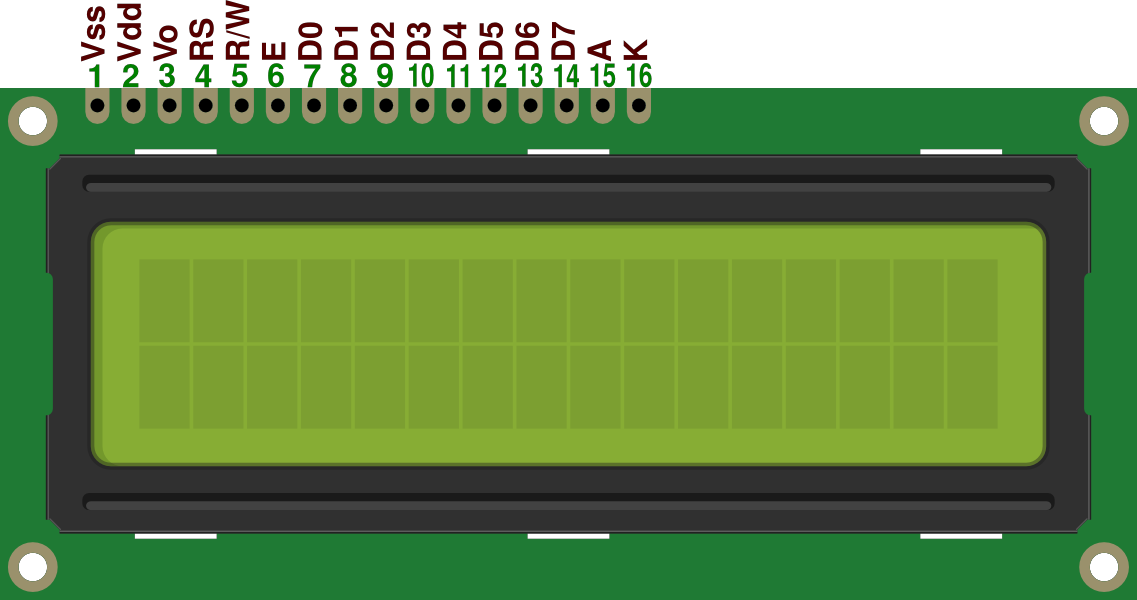
\includegraphics[scale=0.25]{02-hardware/07-lcd162.png}
	\caption{LCD 16x2}
	\label{fig:figura27}
	\end{figure}

La conexión se realiza mediante cuatro pines: alimentación 5V, GND, SCL y SDA.
Además, la placa de adaptación cuenta con un potenciómetro que permite regular
el brillo del LCD.

\begin{figure}[hbtp]
    \centering
    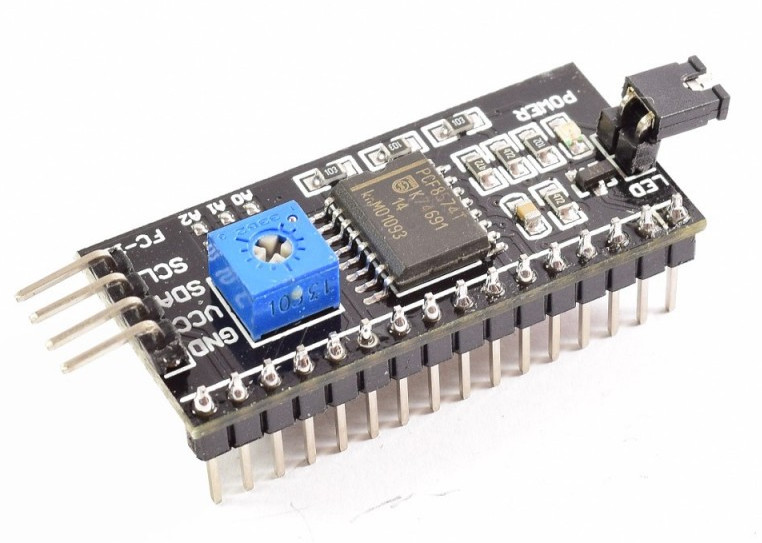
\includegraphics[scale=1]{02-hardware/08-modulo-adaptador-lcd-a-i2c.jpg}
    \caption{Módulo de control de LCD por I2C}
    \label{fig:figura28}
    \end{figure}

\section{Sensor fotoeléctrico OMRON}

Se utiliza un sensor fotoeléctrico para detectar que la pieza ha llegado a cierta posición arbitraria.
Para ello se utiliza el sensor E3JK-R4M de la marca OMRON. Este sensor se encuentra incorporado en la cinta
transportadora del laboratorio. Tiene dimensiones reducidas y tiene una alta capacidad de conmutación. El 
sensor es de tipo retroreflectivo polarizado, lo que permite detectar cuerpos brillantes. Además, posee un
LED de color rojo que se encinede al detectar un objeto.

\begin{figure}[hbtp]
    \centering
    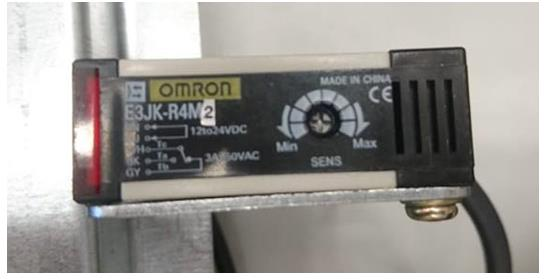
\includegraphics[scale=0.5]{02-hardware/09-omron.png}
    \caption{Sensor fotoeléctrico OMRON E3JK-R4M}
    \label{fig:figura29}
    \end{figure}

\subsection{Conexiones del sensor fotoeléctrico}

El sensor fotoeléctrico cuenta con cinco cables de conexión de diferentes colores:
\begin{itemize}
    \item Marrón. Alimentación entre 12-24V.
    \item Azul. GND.
    \item Blanco. Salida común del relé.
    \item Negro. Salida de relé NA (Normalmente Abierto).
    \item Gris. Salida de relé NC (Normalmente Cerrado).
\end{itemize}

\section{Cinta transportadora con elementos integrados}

En el laboratorio de automática se encuentra una cinta transportadora con todos los elementos integrados,
de modo que el proyecto consiste en definitva en una interfaz entre estos elementos y el robot que le
acompaña.

\begin{figure}[hbtp]
    \centering
    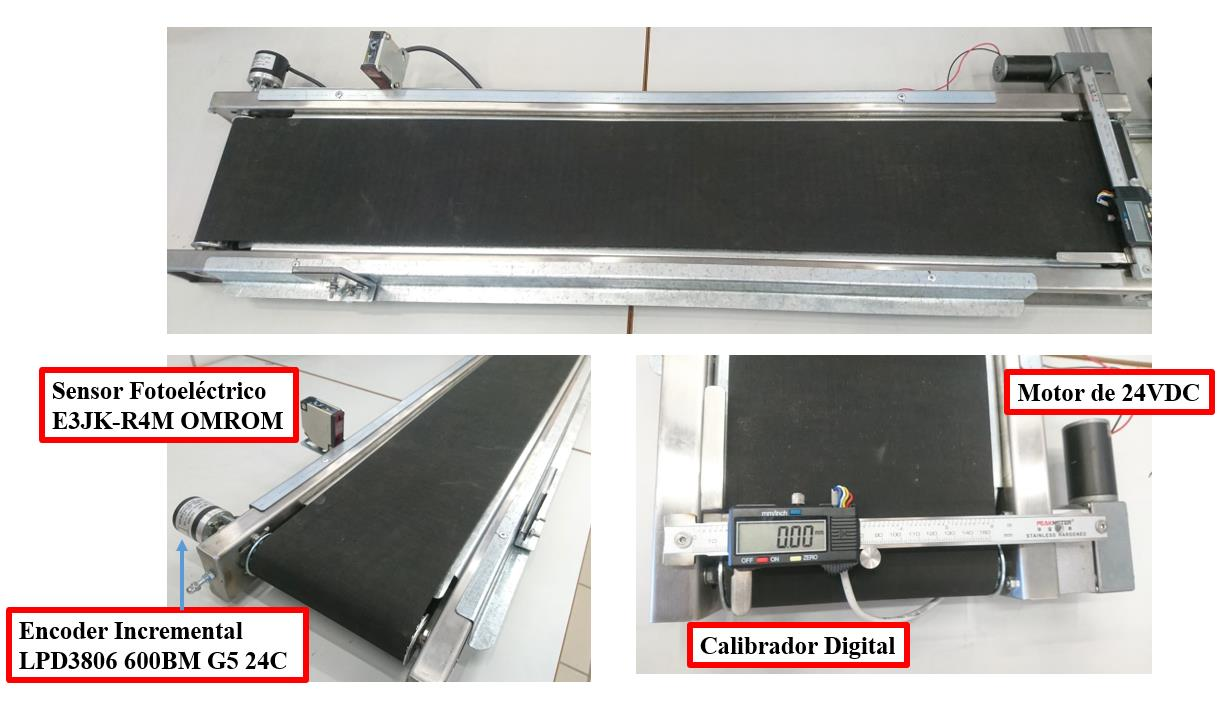
\includegraphics[width=\textwidth]{02-hardware/10-banda.png}
    \caption{Cinta transportadora con elementos integrados}
    \label{fig:figura210}
    \end{figure}

\section{Convertidor CC-CC con salida USB}

Se trata de un pequeño dispositivo que se puede alimentar con un amplio rango de tensiones. En este caso,
se puede alimentar con los 24V que proporciona la controladora del robot. Cuenta con cuatro salidas USB 
(que funcionan a 5V) con las que se puede alimentar la placa de Arduino y toda la electrónica del sistema.

\section{Controladora IRC5C}

El robot ABB IRB120 presente en los laboratorios del departamento cuentan con unas controladoras IRC5C,
que son los dispositivos con los que se tiene que interactuar para comunicar la cinta transportadora con
el robot. Estos dispositivos funcionan a 24V y cuentan con su propia fuente de alimentación. Por otra parte,
cuentan con todas las conexiones necesarias para la realización del proyecto. Entre ellas, una conexión Ethernet
a la que conectar el Ethernet Shield de Arduino.

Por otro lado, cuenta con una placa DSQC 652, que permite la conexión de señales digitales. Estas señales tienen
un nivel lógico de 24V, necesitando un mínimo de 15V para detectar un '1' y un máximo de 5V para detectar un '0',
por lo que las señales que les sean enviadas por esta vía deben ser adaptadas a dichas tensiones.

\section{Optoacoplador TLP621-4}

El circuito integrado TLP621-4 se trata de un chip que cuenta con cuatro aisladores ópticamente acoplados que constan
con un diodo emisor de luz infrarroja y un fototransistor de silicio NPN encapsulado en plástico.

Las principales características son:
\begin{itemize}
    \item Tensión de aislamiento en AC de 5300Vrms.
    \item Rango de temperatura de funcionamiento: -30ºC a 100ºC.
    \item Sin plomo.
    \item Paquete DIP de 16 pines.
\end{itemize}